%% History:
% Pavel Tvrdik (26.12.2004)
%  + initial version for PhD Report
%
% Daniel Sykora (27.01.2005)
%
% Michal Valenta (3.12.2008)
% rada zmen ve formatovani (diky M. Duškovi, J. Holubovi a J. Žďárkovi)
% sjednoceni zdrojoveho kodu pro anglickou, ceskou, bakalarskou a diplomovou praci

% One-page layout: (proof-)reading on display
%%%% \documentclass[11pt,oneside,a4paper]{book}
% Two-page layout: final printing
\documentclass[11pt,twoside,a4paper]{book}   
%=-=-=-=-=-=-=-=-=-=-=-=--=%
% The user of this template may find useful to have an alternative to these 
% officially suggested packages:
\usepackage[czech, english]{babel}
\usepackage[T1]{fontenc} % pouzije EC fonty 
% pripadne pisete-li cesky, pak lze zkusit take:
% \usepackage[OT1]{fontenc} 
\usepackage[utf8]{inputenc}
%=-=-=-=-=-=-=-=-=-=-=-=--=%
% In case of problems with PDF fonts, one may try to uncomment this line:
%\usepackage{lmodern}
%=-=-=-=-=-=-=-=-=-=-=-=--=%
%=-=-=-=-=-=-=-=-=-=-=-=--=%
% Depending on your particular TeX distribution and version of conversion tools 
% (dvips/dvipdf/ps2pdf), some (advanced | desperate) users may prefer to use 
% different settings.
% Please uncomment the following style and use your CSLaTeX (cslatex/pdfcslatex) 
% to process your work. Note however, this file is in UTF-8 and a conversion to 
% your native encoding may be required. Some settings below depend on babel 
% macros and should also be modified. See \selectlanguage \iflanguage.
% \usepackage{czech}  %%%%%\usepackage[T1]{czech} %%%%[IL2] [T1] [OT1]
%=-=-=-=-=-=-=-=-=-=-=-=--=%

%%%%%%%%%%%%%%%%%%%%%%%%%%%%%%%%%%%%%%%
% Styles required in your work follow %
%%%%%%%%%%%%%%%%%%%%%%%%%%%%%%%%%%%%%%%
\usepackage{graphicx}
%\usepackage{indentfirst} %1. odstavec jako v cestine.

\usepackage{k336_thesis_macros} % specialni makra pro formatovani DP a BP
 % muzete si vytvorit i sva vlastni v souboru k336_thesis_macros.sty
 % najdete  radu jednoduchych definic, ktere zde ani nejsou pouzity
 % napriklad: 
 % \newcommand{\bfig}{\begin{figure}\begin{center}}
 % \newcommand{\efig}{\end{center}\end{figure}}
 % umoznuje pouzit prikaz \bfig namisto \begin{figure}\begin{center} atd.
\usepackage{amssymb,amsmath}

%%%%%%%%%%%%%%%%%%%%%%%%%%%%%%%%%%%%%
% Zvolte jednu z moznosti 
% Choose one of the following options
%%%%%%%%%%%%%%%%%%%%%%%%%%%%%%%%%%%%%
% \newcommand\TypeOfWork{Diplomová práce} \typeout{Diplomova prace}
% \newcommand\TypeOfWork{Master's Thesis}   \typeout{Master's Thesis} 
\newcommand\TypeOfWork{Bakalářská práce}  \typeout{Bakalarska prace}
% \newcommand\TypeOfWork{Bachelor's Project}  \typeout{Bachelor's Project}


%%%%%%%%%%%%%%%%%%%%%%%%%%%%%%%%%%%%%
% Zvolte jednu z moznosti 
% Choose one of the following options
%%%%%%%%%%%%%%%%%%%%%%%%%%%%%%%%%%%%%
% nabidky jsou z: http://www.fel.cvut.cz/cz/education/bk/prehled.html

\newcommand\StudProgram{Elektrotechnika a informatika, dobíhající, Bakalářský}
% \newcommand\StudProgram{Elektrotechnika a informatika, dobíhající, Magisterský}
% \newcommand\StudProgram{Elektrotechnika a informatika, strukturovaný, Bakalářský}
% \newcommand\StudProgram{Elektrotechnika a informatika, strukturovaný, Navazující magisterský}
% \newcommand\StudProgram{Softwarové technologie a management, Bakalářský}
% English study:
% \newcommand\StudProgram{Electrical Engineering and Information Technology}  % bachelor programe
% \newcommand\StudProgram{Electrical Engineering and Information Technology}  %master program


%%%%%%%%%%%%%%%%%%%%%%%%%%%%%%%%%%%%%
% Zvolte jednu z moznosti 
% Choose one of the following options
%%%%%%%%%%%%%%%%%%%%%%%%%%%%%%%%%%%%%
% nabidky jsou z: http://www.fel.cvut.cz/cz/education/bk/prehled.html

\newcommand\StudBranch{Výpočetní technika}   % pro program EaI bak. (dobihajici i strukt.)
% \newcommand\StudBranch{Výpočetní technika}   % pro prgoram EaI mag. (dobihajici i strukt.)
% \newcommand\StudBranch{Softwarové inženýrství}            %pro STM
% \newcommand\StudBranch{Web a multimedia}                  % pro STM
% \newcommand\StudBranch{Computer Engineering}              % bachelor programe
% \newcommand\StudBranch{Computer Science and Engineering}  % master programe


%%%%%%%%%%%%%%%%%%%%%%%%%%%%%%%%%%%%%%%%%%%%
% Vyplnte nazev prace, autora a vedouciho
% Set up Work Title, Author and Supervisor
%%%%%%%%%%%%%%%%%%%%%%%%%%%%%%%%%%%%%%%%%%%%

\newcommand\WorkTitle{Galerie fotografií s exportem na webové stránky }
\newcommand\FirstandFamilyName{Pavel Macenauer}
\newcommand\Supervisor{Doc. Ing. Jan Janoušek CSc.}


% Pouzijete-li pdflatex, tak je prijemne, kdyz bude mit vase prace
% funkcni odkazy i v pdf formatu
\usepackage[
pdftitle={\WorkTitle},
pdfauthor={\FirstandFamilyName},
bookmarks=true,
colorlinks=true,
breaklinks=true,
urlcolor=red,
citecolor=blue,
linkcolor=blue,
unicode=true,
]
{hyperref}



% Extension posted by Petr Dlouhy in order for better sources reference (\cite{} command) especially in Czech.
% April 2010
% See comment over \thebibliography command for details.

\usepackage[square, numbers]{natbib}             % sazba pouzite literatury
%\usepackage{url}
%\DeclareUrlCommand\url{\def\UrlLeft{<}\def\UrlRight{>}\urlstyle{tt}}  %rm/sf/tt
%\renewcommand{\emph}[1]{\textsl{#1}}    % melo by byt kurziva nebo sklonene,
\let\oldUrl\url
\renewcommand\url[1]{<\texttt{\oldUrl{#1}}>}




\begin{document}

%%%%%%%%%%%%%%%%%%%%%%%%%%%%%%%%%%%%%
% Zvolte jednu z moznosti 
% Choose one of the following options
%%%%%%%%%%%%%%%%%%%%%%%%%%%%%%%%%%%%%
\selectlanguage{czech}
%\selectlanguage{english} 

% prikaz \typeout vypise vyse uvedena nastaveni v prikazovem okne
% pro pohodlne ladeni prace


\iflanguage{czech}{
	 \typeout{************************************************}
	 \typeout{Zvoleny jazyk: cestina}
	 \typeout{Typ prace: \TypeOfWork}
	 \typeout{Studijni program: \StudProgram}
	 \typeout{Obor: \StudBranch}
	 \typeout{Jmeno: \FirstandFamilyName}
	 \typeout{Nazev prace: \WorkTitle}
	 \typeout{Vedouci prace: \Supervisor}
	 \typeout{***************************************************}
	 \newcommand\Department{Katedra počítačů}
	 \newcommand\Faculty{Fakulta elektrotechnická}
	 \newcommand\University{České vysoké učení technické v Praze}
	 \newcommand\labelSupervisor{Vedoucí práce}
	 \newcommand\labelStudProgram{Studijní program}
	 \newcommand\labelStudBranch{Obor}
}{
	 \typeout{************************************************}
	 \typeout{Language: english}
	 \typeout{Type of Work: \TypeOfWork}
	 \typeout{Study Program: \StudProgram}
	 \typeout{Study Branch: \StudBranch}
	 \typeout{Author: \FirstandFamilyName}
	 \typeout{Title: \WorkTitle}
	 \typeout{Supervisor: \Supervisor}
	 \typeout{***************************************************}
	 \newcommand\Department{Department of Computer Science and Engineering}
	 \newcommand\Faculty{Faculty of Electrical Engineering}
	 \newcommand\University{Czech Technical University in Prague}
	 \newcommand\labelSupervisor{Supervisor}
	 \newcommand\labelStudProgram{Study Programme} 
	 \newcommand\labelStudBranch{Field of Study}
}




%%%%%%%%%%%%%%%%%%%%%%%%%%    Poznamky ke kompletaci prace
% Nasledujici pasaz uzavrenou v {} ve sve praci samozrejme 
% zakomentujte nebo odstrante. 
% Ve vysledne svazane praci bude nahrazena skutecnym 
% oficialnim zadanim vasi prace.
{
\pagenumbering{roman} \cleardoublepage \thispagestyle{empty}
\chapter*{Na tomto místě bude oficiální zadání vaší práce}
\begin{itemize}
\item Toto zadání je podepsané děkanem a vedoucím katedry,
\item musíte si ho vyzvednout na studiijním oddělení Katedry počítačů na Karlově náměstí,
\item v jedné odevzdané práci bude originál tohoto zadání (originál zůstává po obhajobě na katedře),
\item ve druhé bude na stejném místě neověřená kopie tohoto dokumentu (tato se vám vrátí po obhajobě).
\end{itemize}
\newpage
}

%%%%%%%%%%%%%%%%%%%%%%%%%%    Titulni stranka / Title page 

\coverpagestarts

%%%%%%%%%%%%%%%%%%%%%%%%%%%    Podekovani / Acknowledgements 

\acknowledgements
\noindent
Zde můžete napsat své poděkování, pokud chcete a máte komu děkovat.


%%%%%%%%%%%%%%%%%%%%%%%%%%%   Prohlaseni / Declaration 

\declaration{V~Praze dne 16.\,12.\,2011}
%\declaration{In Kořenovice nad Bečvárkou on May 15, 2008}


%%%%%%%%%%%%%%%%%%%%%%%%%%%%    Abstract 
 
\abstractpage
\noindent 
The thesis deals with the implementation of an application called GalleryManager used for multiple-photo management, their organization, editing and also export into a presentation. It is a multiplatform graphical interface application allowing the creation of a tree-structured project consisting of galleries, photos and then editing them both individually and massively. Output is in the form of a web presentation. Emphasis is mainly on the speed of photo processing and efficiency of the algorithms.

\indent 
The application should be designed in a way, that it allows to add additional functionalities to the extent of a complete graphical suite for photo editing. Input format is mainly JPEG and individual adjustments are processed in an 8-bit RGB colour space.

% Prace v cestine musi krome abstraktu v anglictine obsahovat i
% abstrakt v cestine.
\vglue60mm

\noindent{\Huge \textbf{Abstrakt}}
\vskip 2.75\baselineskip

\noindent 
Práce se zabývá implementací programu GalleryManager, sloužícího k hromadné správě fotografií, jejich organizaci, úpravám a následně i exportu do podoby prezentace. Jedná se o multiplatformní grafickou aplikaci, která umožňuje vytvořit si vlastní stromově strukturovaný projekt tvořený galeriemi, fotografiemi a každou pak jak samostnatně, tak i hromadně zpracovávat. Výstupem je webová prezentace. Důraz je kladen predevším na rychlost zpracování fotografií a efektivitu použitých algoritmů.

\indent 
Program by měl být navržen tak, aby do něj šlo přidávat i další funkce až do podoby kompletního grafického studia ke zpracování fotografií. Vstupním formátem fotografií je především JPEG, samotné úpravy jsou pak prováděny v 8-bitovém RGB prostoru.

%%%%%%%%%%%%%%%%%%%%%%%%%%%%%%%%  Obsah / Table of Contents 

\tableofcontents


%%%%%%%%%%%%%%%%%%%%%%%%%%%%%%%  Seznam obrazku / List of Figures 

\listoffigures


%%%%%%%%%%%%%%%%%%%%%%%%%%%%%%%  Seznam tabulek / List of Tables

\listoftables


%**************************************************************

\mainbodystarts
% horizontalní mezera mezi dvema odstavci
%\parskip=5pt
%11.12.2008 parskip + tolerance
\normalfont
\parskip=0.2\baselineskip plus 0.2\baselineskip minus 0.1\baselineskip

% Odsazeni prvniho radku odstavce resi class book (neaplikuje se na prvni 
% odstavce kapitol, sekci, podsekci atd.) Viz usepackage{indentfirst}.
% Chcete-li selektivne zamezit odsazeni 1. radku nektereho odstavce,
% pouzijte prikaz \noindent.

%**************************************************************

% Pro snadnejsi praci s vetsimi texty je rozumne tyto rozdelit
% do samostatnych souboru nejlepe dle kapitol a tyto potom vkladat
% pomoci prikazu \include{jmeno_souboru.tex} nebo \include{jmeno_souboru}.
% Napr.:
% \include{1_uvod}
% \include{2_teorie}
% atd...

%*****************************************************************************

\chapter{Úvod}

\noindent
V současné době je na trhu velké množství grafických editorů, programů pro správu fotografií a těch, které kombinují obojí. Z komerčních produktů jsou nejznámější rozsáhlé programové balíky Photoshop a Lightroom od Adobe Systems Inc. V České Republice se velmi dobře prosadil i mnohem levnější Zoner Photo Studio. Bezplatně je možné využívat služeb Google Picassa nebo IrfanView. Některé z nich za sebou mají již desítky let vývoje, teamy vývojářů, a tak jim nelze příliš konkurovat.

\indent
GalleryManager je jednoduchým grafickým editorem a správcem fotografií včetně veškerých popisů. Tuto aplikaci do budoucna plánují integrovat do správy vlastních webových stránek, zaměřených na cestovatelskou fotografii PhotographicAtlas.com a FotoAtlas.cz. Není tak cílem implementovat pokročilé algoritmy pro úpravu fotografií, které již nabízejí existující softwary, zameřené na práci s velkými soubory a tisk. Naopak je kladen důraz na rychlost a efektivitu pro potřeby webové prezentace.

\indent
Dokumentární nebo reportážní fotografové, pro které je GalleryManager určen, nespravují své fotografie jednotlivě, ale jako celé série. Cílem je zpřístupnit i neobrazové informace vkladáné fotoaparáty do fotografie (na příklad údaje o nastavení fotoaparátu, místě a času pořízení snímku a další).

\indent
Aktuálně je aplikace navržena tak, aby výstupem byla nezávislá webová stránka, kterou lze použít pro vlastní prezentaci na internetu.

\indent
Tato práce je implementační, nikoliv rešeršní, proto dokumentace bude popsána především z programátorského hlediska, popisující postup při tvorbě aplikace a možnosti použitých knihoven. Vzhledem k tomu, že bych se i do budoucna chtěl věnovat úpravám obrazu a nadále rozšířovat aplikaci o další možnosti, budou popsány jednotlivé algoritmy pro úpravu fotografií, jejich výhody, nevýhody a srovnání s jinými obecně známými.

%*****************************************************************************

\chapter{Popis problému, specifikace cíle}
\section{Cíle práce}

\noindent
Hlavním cílem této práce je vytvořit grafický editor, který umožní organizovat, popisovat a nakonec exportovat fotografie do podoby webové prezentace. Nejedná se o práci, která bude prezentována jako hotový program, ale spíše jako framework pro správu a úpravy fotografií, který půjde dále rozšiřovat.

\indent
Zpracování obrazu a informací spojených s fotografií je natolik rozsáhlé téma, že přesahuje rozsah bakalářské práce, časové možnosti a i znalosti jediného člověka. Cílem aplikace GalleryManager je vytvořit:

\begin{itemize}
\item grafické uživatelské rozhraní
\item stromovou strukturu podsložek (galerií) a jednotlivých fotografií
\item možnost každou galerii a fotografii popisovat, do budoucna by měla být struktura přizpůsobena, aby šla rozšiřovat
\item automatické vkládání informací z EXIF údajů fotografie
\item základní grafické úpravy - jas, kontrast, transformace obrazu, ...
\item export projektu do standardních formátů - XML, HTML+CSS a možnost ho ukládat a opět načítat
\item multiplatformní podporu aplikace
\end{itemize}

\section{Podoba práce vzhledem k vytyčeným cílům}
\noindent
Jedná se o standartní grafickou aplikaci psanou v jazyce C++. Průběh práce s programem, při zpracování a organizaci vlastních fotografií fotografií vypadá takto:
\begin{itemize}
% % 1., 2., ...
\item spustí se program GalleryManager obsahující prázdný projekt bez jakýchkoliv podsložek
\item uživatel má možnost nahrát projekt, se kterým pracoval již v minulosti, obsahující podsložky a fotografie
\item v rámci projektu lze vytvářet nové podsložky (galerie) nebo upravovat již existující
\item poté do existujících nebo nově vytvořených podsložek naimportuje uživatel nové fotografie
	\subitem během importu fotografií se načtou a zobrazí EXIF informace
	\subitem bude možné přidávat další popisky
	\subitem při rozkliknutí složky se zobrazí její obsah - podložky jako obálky a fotografie jako malé náhledy
	\subitem při rozkliknutí fotografie se zobrazí fotografie v plném rozlišení v prostředí pro úpravu
\item projekt lze ukládat ve formátu XML
\item projekt lze exportovat ve formátu HTML do podoby webové prezentace, při čemž vzhled se určí pomocí vložené CSS šablony
\item CSS lze libovolně vytvářet na základě popsané HTML struktury a tak vkládat vlastní design
\end{itemize}

\section{Existující implementace}
\noindent
Již existující implementace existují v několika kategoriích. Komerční, nekomerční, grafické editory a aplikace pro správu fotografií. Mezi komerční software patří především zástupci rodiny produktů Adobe Systems Inc. - Adobe Photoshop, jeho odlehčená verze Adobe Photoshop Elements a Adobe Lightroom. Následně do nižší cenové kategorie zapadá Zoner Photo Studio, populární především v České Republice. Od komerčních aplikací, které se zabývají především pokročilými úpravami obrazu, se nekomerční soustředí spíše na organizaci a prohlížení fotografií. K nim lze zařadit Google Picassa, IrfanView a software přiložený ke správě uživatelského účtu na Rajce.cz. Žádný z těchto programů nedistribuje své zdrojové kódy, proto jediným zdrojem informací jsou uživatelské zkušenosti se samotnými aplikacemi.

\subsection{Komerční software}
\noindent
Nejznámějším specializovaným softwarem pro úpravu jednotlivých fotografií, ale i pro tvorbu grafiky je bezpochyby Adobe Photoshop od Adobe Systems Inc. Tento program umožňuje obrovské možnosti zpracování obrazu na úrovní až 32-bitové barevné hloubky a v současné době nemá na trhu grafických aplikací konkurenci. Mimojiné existuje i jeho odlehčená varianta Adobe Photoshop Elements, která neobsahuje tolik specializovaných funkcí pro úpravu obrazu. 

\indent
Zajímavější aplikací je Adobe Lightroom. Neumožňuje tolik pokročilých úprav, jako právě Photoshop, ale lze v něm zpracovávat více fotografií naráz, ty následně organizovat, upravovat jejich fotografické informace a výsledný projekt i exportovat. Nevýhodou je, že jej nelze integrovat do vlastních projektů a napojit ho na vlastní webový server, k čemuž je GalleryManager do budoucna zamýšlen.

\indent
Především v České Republice se využívá ještě Zoner Photo Studia, které nemá tolik možností je podobné spíše Adobe Photoshopu, neobsahuje ale tolik funkcí a je pro uživatele atraktivní spíše svou jednoduchostí, cenou a českým autorem.

\indent
Každá z těchto aplikací je zaměřena především na úpravy obrazu, které jsou u GalleryManageru pouze doplňkem. Budeme tak porovnávat výstup z těchto programů a z naší implementace na vzorových fotografiích především z hlediska obrazové kvality upravených fotografií.

\subsection{Nekomerční software}
\noindent
Druhou skupinou existujících implementací je nekomerční software, který slouží především jako podpora nebo nadstavba služeb poskytovaných webovými servery. Česká webová stránka rajce.cz umožňuje uživatelům sdílet své fotografie v podobě galerií. Ke svému účtu poskytuje software, pomocí kterého si uživatel vytvoří galerii, pojmenuje ji, popíše a na svém počítači vybere fotografie, které do něj chce vložit. Program pak už samotné fotografie zmenší na velikost náhledů ve webové prezentaci na internetových stránkách www.rajce.cz. Samotné fotografie lze pouze otočit po 90-ti stupních a pojmenovat. Není možné je jakkoliv jinak upravovat nebo číst jejich EXIF údaje v širším měřítku.

\indent
IrfanView je naopak spíše jednoduchým prohlížečem fotografií. Umožňuje oproti komerčnímu softwaru pouze základní grafické úpravy. Jeho hlavní předností a záměrem je zobrazovat fotografie, proto podporuje většinu dnes používaných grafických formátu a umožňuje spustit slideshow prezentaci.

\indent
Posledním a nejpodobnějším softwarem je Google Picasa, který je se spuštěním sociální sítě Google+ je využíván pro synchronizaci fotografií s vlastním uživatelským účtem, ale lze jej používat i samostatně pro grafické úpravy. Galerie se zde vytvářejí přímo v podobě systémových složek, které si Picasa neustále za svého běhu indexuje. Uživatel tak má přehled o všech svých fotografiích na pevném disku. Zajímavé je, že každou chvíli si určitou část využívané paměti uvolní a nezabírá tak obrovské množství paměti, jaké by člověk očekával od programu, který si neustále vytváří náhledy.
\indent
Sociální sítě dnes slouží především k masovému sdílení vlastních informací. Stejným způsobem pohlíží i Picasa na fotografie. Je přizpůsobena pro běžného uživatele, kterému stačí jednoduché úpravy fotografií, může je synchronizovat s Google+ a prohlížet téměř každý dnes používaný formát. Neumožňuje číst velké množství EXIF informací a dokumentovat tak dostatečně své galerie.

%*****************************************************************************
\bibliographystyle{csplainnat}
%bibliographystyle{plain}
%\bibliographystyle{psc}

\chapter{Analýza a návrh řešení}
\section{Volba programovacích jazyků a knihoven}
\noindent
GalleryManager je mimojiné i grafickým editorem. Jeden z požadavků je upravovat a obsluhovat velké množství fotografií současně. Potřebujeme tak co nejrychlejší jazyk s velkým množstvím dostupných knihoven, především pro tvorbu GUI, úpravu obrazu a čtění EXIF dat. Zároveň musí být objektově orienovaný a mapovat tak koncept reálného světa. Pro nás je důležité vytvářet strukturu galerií a fotografií, kde každá galerie v sobě může obsahovat opět další galerie a fotografie. 

\indent 
Zvolen byl programovací jazyk C++, který všechny tyto požadavky splňuje. Jeho nevýhodou je, že oproti výše-úrovňovým jazykům jako Java, se zde programátor musí starat o správu paměti a hodně funkcí, které by byly jinak obsaženy v základních knihovnách, psát ručně.

\indent
Jednotlivé použité knihovny je třeba analyzovat po částech aplikace, kde každá by měla být na druhé co nejméně závislá. Nechceme, aby docházelo k tomu, že při změně části kódu bude třeba přepisovat zbytek aplikace.

\subsection{Grafické uživatelské rozhraní}
\indent
Ke tvorbě grafického uživatelského rozhraní je použit široce rozšířený framework Qt od Nokie. K jeho výběru vedlo hned několik výhod. Je volně ke stažení pod licencí LGPL v2.1, umožnující volné používání pro nekomerční účely. Z programátorského hlediska má přehlednou dokumentací, je multiplatformní, tudíž GUI a signály nejsou vázány na operační systém a umožňuje obrovské množství dalších funkcí spojených nejen s úpravou obrazu a GUI. Jeden z problémů, který musíme řešit, je vykreslování obrazu po provedení úpravy. Qt umožňuje vytvořit prázdný obraz a vykreslovat do něj pixel po pixelu, kterému se zadají pouze barevné informace.

\subsection{Zpracování obrazu}
\indent
Knihovny Qt umožňují pouze jednoduché možnosti zpracování obrazu. Za jeden z cílů jsme si zvolili možnost do budoucna rozšiřovat GalleryManager směrem grafického editoru. Především tak pracovat i ve více bitových barevných hloubkách, krom 8-bit i 16-bit a v jiných barevných prostorech, nejen RGB, ale i LAB či CMYK. K načítání obrazových dat jsme tak zvolili open-source knihovnu Boost::GIL od Adobe, která je používána i v jeho komerčních produktech. To nám umožňuje daleko větší režii nad úpravou obrazu, než-li by nám poskytlo samotné Qt. Úpravy jsou pak z důvodu požadavků na efektivitu a vzdělávacích účelů, implementovány pomocí adekvátních algoritmů za pomoci Boost::GIL a standartního C++.

\subsection{Čtení EXIF údajů}
\noindent
Většina digitálních fotoaparátů nebo smartphonů dnes ukládá metadata o pořízeném snímku, jakými jsou čas, clonové číslo, použitý fotoaparát, objektiv i jeho ohnisko, přímo do fotografie ve formátu EXIF. Krom technických parametrů mezi nimi nemusí chybět ani GPS informace, má-li dané zařízení možnost určovat vlastní polohu. Uživatel, ani programátor se tak nemusí starat o ruční vkládání dat, ale vše je získáváno přímo z fotografie.

\indent
K implementaci v prostředí C++ existují knihovny libexif a exiv2. Exiv2 je oproti libexif napsána v C++ a umožňuje číst i další standarty k uchovávání metadat - XMP\footnote{Extensible Metadata Platform - standart od Adobe Systems Inc. k ukládání informací především v PDF, fotografiích, grafice} a IPTC\footnote{Information Interchange Model od International Press Telecommunications Council je další ze standartů na úkládání dodatečných informací o souborech}. Její nevýhodou je, že obsahuje závislosti na jiných knihovnách, jmenovitě zlib, gettext, libiconv a Expat, čímž značně přesahuje měřítko ve kterém chceme implementovat podporu metadat, zvětšuje i velikost celé práce a za cíl jsme si aktuálně zvolili číst pouze nejpoužívanější formát EXIF.

\indent
Druhou knihovnou, napsanou v jazyce C, je libexif\cite{libexif}, kterou používáme i v této práci. Při integraci do moderního C++ prostředí toto výtváří úskalí především v konceptu C++, které už není zdaleka tak nízkoúrovňové jako C. Její výhodou je, že nepotřebuje žádné další závislosti. U GalleryManageru požadujeme pouze zobrazení všech EXIF informací o fotografii, které by mohli uživatele zajímat. Knihovna je tak pro naše účely zcela dostačující.

\subsection{Výstup z programu}
\noindent
Výstup z programu je ve 2 podobách. První z nich je ukládání samotného projektu do formátu, ze kterého půjde opět lehce načítat. K tomu je dnes hojně rozšířen jazyk XML. Výhodou využití frameworku Qt je, že v sobě zahrnuje i knihovny pro generování a čtení XML, pomocí kterých můžeme vygenerovat soubor obsahující všechny potřebné informace k uložení a zpětnému načtení celého projektu.

\indent
Druhou a zajímavejší formou výstupu je vygenerování webové prezentace. HTML je velmi podobné XML, proto je použit opět stejný generátor, jako pro ukládání projektu, tentokráte pouze s HTML výstupem. Design prezentace je řešen už předem napsanými CSS styly, které se přiloží k webové stránce. CSS je zde zvoleno především z důvodu jeho rozšířenosti a nezávislosti na HTML kódu. Poskytneme tak pouze kostru webové stránky, které se design vytvoří dodatečně. Součástí práce bude jeden výchozí styl, další si budou mít možnost uživatelé vytvořit sami.


\section{Prostředí pro vývoj aplikace}
\noindent
Ke tvorbě programu je použito volně dostupné vývojové prostředí Qt Creator běžící na platformě Windows, které plně poporuje značení C++ syntaxe a čtění obsahu jednotlivých tříd. Navíc obsahuje i integrovanou dokumentaci frameworku Qt. K jeho volbě vedla nejeden již zmíněná dokumentace frameworku Qt, ale i rychlost a jednoduchost používání, na rozdíl od běžně využívaného Microsoft Visual Studia, obsahujícího velké množsví funkcí, které programátor nevyužije. Jako C++ kompilátor využívá Qt Creator systém MinGW.

\section{Správa a záloha kódu}
\noindent
Při tvorbě větších softwarových projektů je třeba spravovat vlastní kód. Především z důvodu, aby bylo vidět, jaké dílčí úkoly už jsou hotové a jaké je třeba stále dodělat, se založil veřejný repositář. Z důvodu jednoduché instalace, kvalitního zázemí internetového serveru github.com a možnosti založit si zdarma účet, jsme se přiklonili k reviznímu systému Git s grafickou nadstavbou pro Microsoft Windows GitTortoise \footnote{repositář je k nalezení na adrese https://github.com/macicek/MGalleryManager-v2}. Zdrojové kódy jsou volně k dispozici, aby nenarušovaly licenční podmínky používaných knihoven. Zároveň slouží repositář i k záloze dat v případě, že by došlo k jejich ztrátě v průběhu vypracovávání bakaláršké práce.

\section{Struktura ukládaných informací}
\noindent
Základní strukturou celého programu je projekt. Ten následně obsahuje libovolné množství galerií, které v sobě můžou obsahovat další galerie nebo fotografie. Vytváříme tak stromovou strukturu galerií a fotografií o neomezené hloubce. Podmínkou je, že každá fotografie musí být součástí nějaké galerie.

\indent
Každá galerie nebo i fotografie o sobě obsahuje popisné informace, které získáváme ze dvou zdrojů. Prvním je pojmenování a popsání každé fotografie či galerie při jejím vytvoření nebo importu. Dalším zdrojem informací jsou EXIF data, ze kterých budeme zobrazovat clonové číslo, čas, ISO, model fotoaparátu, objektiv a jeho ohniskovou vzdálenost, tedy všechný potřebné, aby si uživatel udělal představu o parametrech nastavených při pořízení fotografie.

\section{Zobrazování obsahu galerií a návrh GUI}
\noindent
Grafické uživatelské rozhraní je rozděleno na 2 části - levou a pravou. V levé nalezneme prvky pro správu projektu a zobrazování informací. Zároveň i  ovládací tlačítka k editaci, mazání, importu či vytváření nových galerií. V pravé se pak při kliknutí na danou galerii nebo fotografii (v levé části), zobrazí buď obsah galerie nebo prostředí pro editaci fotografie. Lépe vše popíše diagram \ref{fig:layout}.

\begin{figure}[ht]
\begin{center}
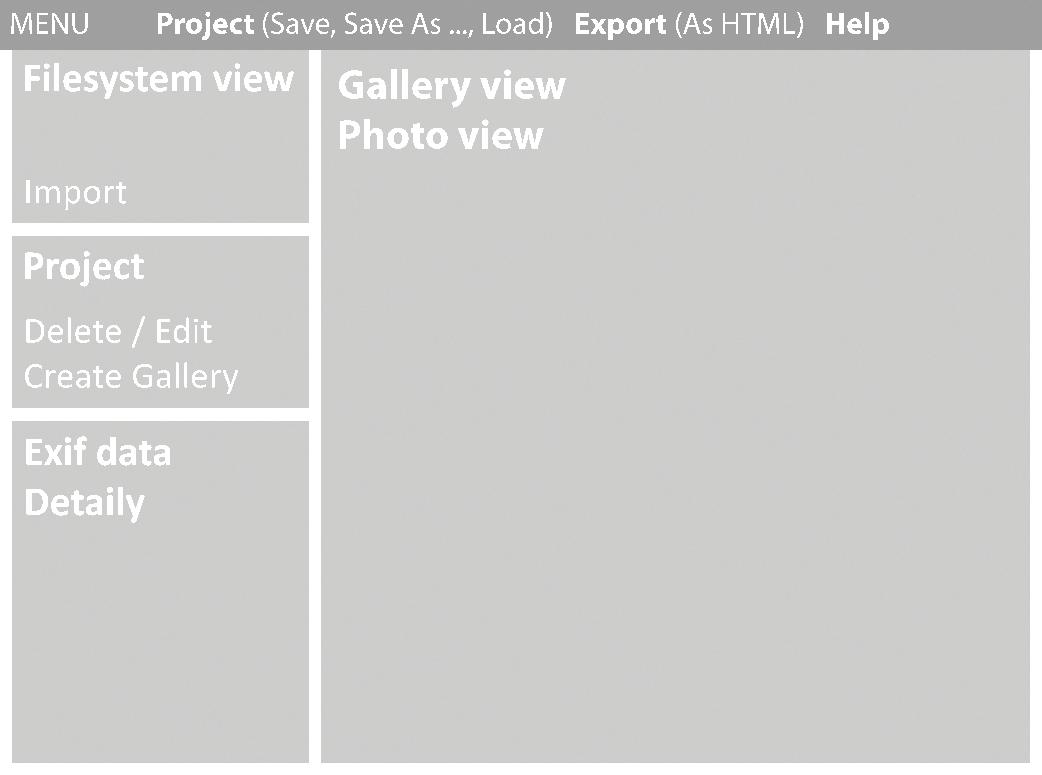
\includegraphics[width=7cm]{figures/layout}
\caption{návrh rozložení aplikace}
\label{fig:layout}
\end{center}
\end{figure}

\indent
V horní části aplikace se nachází menu, které obsahuje možnost ukládat a načítat projekt, export do podoby webové prezentace nebo pomoc odkazující na dokument, v případě, že by si uživatel nevěděl rady.

\section{Dostupné grafické úpravy a práce s pamětí}
\noindent
Úprav, které můžeme aplikovat na obraz, je neomezené množsví. Musíme tak zvolit takové, které běžný uživatel spíše použije. Nejčastěji používanými úpravami jsou jas a kontrast, které jsou schopny oživit barvy a zvýraznit tak původně nezajímavou fotku. Dále GalleryManager implementuje úpravu sytosti. V případě, že umíme fotografie odsytit, můžeme jednoduše přidat možnost převodu do černobílé.

\indent
Nejsou to pouze barvy, které většinou chceme upravovat, často se jedná i o změnu velikosti, aby fotografie nezabírala tolik prostoru nebo rotaci, v případě že je ku příkladu horizont na křivo. Ke každé úpravě zároveň budeme chtít zachovávat její historii, aby ji šlo navrátit do původního stavu v případě, že se úprava nebude líbit.

\indent
Při zpracování obrazu se pracuje s obrovským množstvím dat, proto nastává problém v případě, že chceme upravovat velké množství fotografií současně a zároveň udržovat informace o jejich úpravách. Některé úpravy můžou být destruktivní, tudíž už není možno zrekonstruovat původní snímek zpětným použítím zvolené úpravy. Minimálním množstvím, které tak musíme ukládat je obraz každé úpravy tvořený všemi pixely. S každou další úpravou je méně pravděpodobné, že se uživatel vrátí zpět, proto omezíme počet uložených kroků na předem danou konstantu. Zároveň už není potřeba GUI prvků pro úpravu obrazu v případě, že pracujeme s jiným, proto uvolníme paměť vždy, když už editor nebudeme potřebovat. Naopak malé náhledy fotografií při zobrazení galerie zabírají minimum paměti a očekáváme, že galerií nebude tolik, ale bude mezi nimi uživatel často přecházet. Ponecháme tak veškeré náhledy v paměti až do vypnutí programu.

%*****************************************************************************
\chapter{Realizace}
\noindent
V následující kapitole rozebereme jednotlivé moduly aplikace a jejich implementaci.

\section{Vnitřní informační struktura}
\noindent
Jednotlivé galerie můžou vždy obsahovat buď fotografie nebo další galerie, kde každá je reprezentována vlastní třídou - MGallery, MPhoto. Aby bylo možné uchovávat záznamy o obou třídách současně, dědí obě ještě MObject. Takto lze projekt jednoduše rožšířit o další entity, kterými můžou do budoucna být třeba filmy a implementovat tak třídu MMovie, aniž by se výrazně měnila vnitřní struktura.

MPhoto a MGallery slouží především ke grafickému zpracování. Zeměpisné nebo i fotografické údaje o jednotlivých galeriích a fotografiích jsou řešeny samostatnými třídami. MObject obsahuje strukturu MGPSInfo se zeměpisnými informacemi, společnými jak pro fotografie, tak i pro galerie. Každá galerie a fotografie pak obsahuje ještě struktry MGalleryInfo a MPhotoInfo.

\section{Grafické uživatelské rozhraní}
\noindent
K tvorbě uživatelského rozhraní byl použit framework Qt. Hlavní problémy, které zde musíme řešit, jsou propojení vnitřních struktur uchovávajících informace o fotografiích a galeriích do GUI tříd a vykreslování náhledů během provádění úprav.

\indent
Obsah celého projektu je zobrazován hned na několika místech. Nejprve je třeba zobrazit celou strukturu jako strom, tak aby šlo jednoduše přecházet mezi galeriemi a fotografiemi. Druhým místem je pak hlavní okno, ve kterém se zobrazují náhledy fotografií v aktivní galerii nebo editační prostředí, je-li aktivní pouze samostatná fotografie. Provedeme-li pak úpravu na jakémkoliv z těchto míst, je třeba ji aplikovat i na ostatní.

\section{EXIF údaje fotografií}
\indent
Abychom mohli načíst úspěšně všechna potřebná data, je třeba pochopit strukturu, ve které jsou ukládána. EXIF je založený na formátu JPEG. Data takového obrázku začínají sekvencí 0xFFD8 a končí 0xFFD9. Mimojiné uvnitř existují sekvence značené podobně, konkrétně 0xFF-- nazývané Markers. Markery od 0xFFE0 do  0xFFEF jsou nazývané Application Markers a značí data zaznamenaná uživatelskými aplikaci. EXIF začíná Application Markerem APP1 (0xFFE1), následují různé hlavičky a za nimi IFD0\footnote{Image File Directory} a IFD1, což jsou námi požadované EXIF informace. IFD0 obsahuje informace jakými jsou šířka, výška, ale i offsety na jednotlivé informační položky mezi kterými je i tzv. ExifIFD. To je podsložka IFD0 obsahující veškeré dostupné fotografické informace. Offsety končí odkazem na následující IFD, tedy IFD1 obsahující náhled obrázku. Dále pokračuje datová část na kterou ukazovaly jednotlivé offsety.

\indent
Při čtení EXIFů musíme nejdříve zvolit správné IFD, ve kterém vybereme potřebný tag. Samotné čtení už za nás řeší funkce knihovny libexif \verb|exif_content_get_entry|.

\begin{table}
\begin{center}
\begin{tabular}{|l|r|}
\hline
& APP1 Marker\\
& ... \\
\hline
IFD0 & Image width \\
& Image height \\ 
& ... \\
& ExifIFD offset \\
& GPS offset \\ 
& IFD1 offset \\
& Data \\
\hline
IFD1 & Compression \\
& Resolution \\
\hline
\end{tabular}
\end{center}
\caption{struktura EXIF dat}
\label{tab:tabexif}
\end{table}

\section{Úprava fotografií}
\noindent
Při rozkliknutím detailů jednotlivých fotografií umožňuje GalleryManager grafické úpravy. Ty probíhají nad 8-bitovým RGB prostorem\footnote{Každá barva (červená, zelená, modrá) má 256 úrovní (od 0 do 255), můžeme tedy nakombinovat až $256^{3}=16777216$ různých barev.}. Ke zpracování obrazu jsme zvolili knihovnu boost::GIL\cite{boostgil} od Adobe Systems Inc. GIL nám umožnuje nahlížet na fotografii pomocí dvou datových typů, jako obraz, čili image nebo jako pohled - view. Obraz obsahuje kompletní informace o fotografii, kdežto pohled je pouze jednoduchá struktura uchovávající informace o samotných pixelech. Je proto daleko výhodnější provádět úpravy nad pohledem.

\indent
Jak již bylo zmíněno, GUI je řešeno pomocí frameworku Qt, který také obsahuje třídy pro práci s obrazem, ty jsou ale velice omezené a pro budoucí rozšířování práce nedostatečné. Propojení mezi zpracováním obrazu a vykreslováním náhledu je řešeno přes zkopírování jednotlivých pixelů z obrazu v boost::GIL do QImage, Qt třídy vymezené pro práci s obrazem. QImage už lze jednoduše zobrazit v GUI.

\indent
GalleryManager umožňuje následující úpravy - kontrast, jas, změna sytosti, otočení, transformace velikosti a převod do černobílé.

\subsection{Kontrast}
\noindent
Kontrast nám určuje viditelnost věcí, tedy rozdíl v jasu jednotlivých barev obrazu. GalleryManager využívá následujícího výpočtu na množině reálných čísel: pro každý pixel zvlášť vezme jeho hodnoty RGB, které se pohybují v rozmezí 0 až 255. Od nich odečtě 127 (polovinu maximální hodnoty 255). Vyjde nám odchylka od střední hodnoty. Tu pak vynásobíme koeficientem, kterým chceme změnit kontrast, a k výsledku opět přičteme 127. Ten je převeden zpět na celé číslo a omezen na hodnotu v intervalu <0, 255>. Pokud výsledek před převodem neležel v tomto intervalu, dochází ke ztrátě barevné informace. V extrémních případech, využijeme-li obrovského koeficientu kontrastu, narostou nebo naopak klesnou jednotlivé barevné složky pixelu natolik, že můžou dosahovat pouze hodnot 0 nebo 255. Z původních různobarevných ploch tak vznikají plochy jednobarevné a zpětným snížením kontrastu už nelze vrátit obraz do původního stavu.

\subsection{Jas}
\noindent
Jas se také označuje jako světlost obrazu, tedy jak blízko jsou jednotlivé barvy bílé. Jeho implementace je celkem jednoduchá. RGB je aditivní barevný model, kde jednotlivé barvy přičítáme. Na rozdíl na příklad od CMY(K), kde je naopak odečítáme. U RGB to znamená, že při nulových hodnotách barev (0, 0, 0) dostáváme černou. Naopak při maximálních hodnotách (255, 255, 255) bílou. Jas tak zvyšujeme přičítáním zvolené konstanty ke všem třem složkám a snižujeme odečítáním.

\subsection{Sytost a převod do černobílé}
\noindent
Lidské oko vnímá sytost každé barvy jinak, proto musíme každou měnit v poměru ke koeficientu, kterým ji člověk vnímá. Toto zjednodušuje barevný model HSV\footnote{Hue Saturation Value - Odstín Sytost Hodnota}\cite{graphmodel}, který má sytost jako jednu ze svých složek. Stačí tak převést každý pixel do barevného prostoru HSV, upravit sytost a převést zpět.

\indent
HSV modeluje způsob, kterým pracují výtvarníci. Nejprve vyberou odstín barvy, který chtějí použít a následně přimíchávají černou nebo bílou, ke ztmavení resp. zesvětlení. Výběr odstínu můžeme pozorovat na obrázku \ref{fig:hsv}, kde odstín H je dán úhlem a sytost S vzdáleností od středu.

\begin{figure}[ht]
\begin{center}
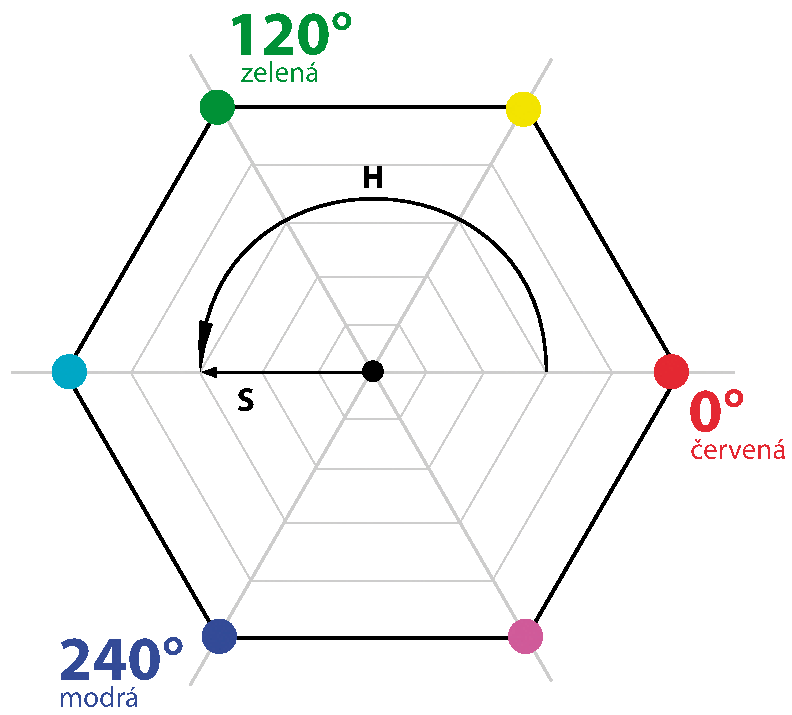
\includegraphics[width=6cm]{figures/hsv}
\caption{hodnoty HS barevného prostoru HSV}
\label{fig:hsv}
\end{center}
\end{figure}

\indent
Převod do HSV nicméně není bezproblémový. Můžeme si všimnout, že v případě, kdy je vzdálenost od středu (sytost) nulová, není možné určit odstín a taková barva je nedefinovaná. K tomu dochází v případě, že se jedná o odstín šedé. V modelu RGB tak mají dílčí barevné složky stejné hodnoty. Převod nám nejlépe popíše následující pseudokód:

\begin{verbatim}
min         = min(red, green, blue)
max         = max(red, green, blue)

value       = max
saturation  = (max-min)/max

if saturation == 0
    hue = UNDEFINED
else
    diff = max - min
    if max == red
        hue = (green - blue) / diff
    else
    if max == green
        hue = 2 + (blue - red) / diff
    else
    if max == blue
        hue = 4 + (red - green) / diff

    hue = hue * 60
    if hue < 0
        hue = hue + 360
\end{verbatim}

\indent
Můžeme pozorovat, že při určování odstínu dělíme rozdílem maximální a minimální hodnoty RGB. V případě šedé jsou všechny tři barvy stejné a rozdíl je nulový. V definičním oborou reálných čísel tak není výpočet definován.

\indent
Sytost se mimojiné dá chápat i jako intenzita nebo čirost dané barvy, jinými slovy ji lze snižovat přidáváním bílé, kdy se barva stává zakalenější. Hodnota V naopak jako odchylka od černé, jejíž přídáváním získáváme intenzivnější dojem. Na základě maximální hodnoty RGB pak určíme v jaké třetine barevného kola se barva nachází. Kterým směrem a o jakou hodnotu barvu posuneme určíme rozdílem sousedních barev.

\indent
Převod do černobílé se provádí snížením sytosti na nulu. U barev, které mají jednu RGB složku nulovou a další 255, tedy maximální, dostaneme vždy bílou. Na \ref{fig:hsv} se jedná o barvy na okraji šestiúhelníku. Nevýhodu tohoto přístupu i přes jeho matematickou správnost je, že tak vznikají bílé plochy, které lidské oko vnímá jako vypálené.

\subsection{Rotace a transformace}
\indent
Rotace je v GalleryManageru řešena přes maticové násobení za pomoci matematického rozšíření knihovny boost::GIL. Nejprve je třeba vygenerovat rotační matici \cite{wiki:rotation}, kterou následně ponásobíme jednotlivé souřadnice. Nastává však problém, že rotace probíhá kolem souřadnic [0, 0], tedy dolního-levého rohu a obraz se dostane mimo plátno. Musíme tak nejprve přízpůsobit velikost plátna a výsledek následně i posunout.

\indent
Boost::GIL využívá matic 3x2, které jsou ve skutečnosti maticemi 3x3, kde poslední řádek je vždy [0 0 1], protože veškeré úpravy probíhají ve 2D prostoru. To nám umožňuje provádět nejen rotaci, ale i translaci pomocí maticového násobení. Stačí tak vygenerovat jednu transformační matici, kterou aplikujeme na každou souřadnici \cite{wiki:affine}. Výpočet probíhá následovně:
$$
\begin{bmatrix}
cos\alpha & -sin\alpha & 0 \\
sin\alpha & cos\alpha & 0 \\
0 & 0 & 1
\end{bmatrix}
\begin{bmatrix}
1 & 0 & t_{x} \\
0 & 1 & t_{y} \\
0 & 0 & 1
\end{bmatrix}
\begin{bmatrix}
x \\
y \\
0
\end{bmatrix}
$$

\indent
Hodnoty $t_{x}$ a $t_{y}$ se získávají funkcemi sin a cos na základě toho, jak se každý roh plátna natočil. Výpočet je různý pro každý kvartál rotace.

\indent 
Při transformaci obrazu, tedy změně jeho velikosti, dochází k jeho deformaci. Je tedy třeba vypočítat výslednou barvu každého nového pixelu. K tomu existuje více metod, kde každá má své výhody i nevýhody. GalleryManager využívá bilineárního vzorkování \cite{wiki:bilinear}, které dosahuje nejlepších výsledků, jsou-li rozměry výsledného obrazu maximálně dvakrát menší nebo větší. Pro srovnání se vzorkováním dle nejbližšího souseda, kde se vybírá vždy barva nejbližšího pixelu, zde barvy průměrujeme, a proto dosahujeme plynulejších přechodů.

\indent
Bilinineární vzorkování používá 4 okolní pixely, jejichž barvu zprůměruje na základě vzdálenosti od výsledného pixelu. Představíme-li si obraz jako mřížku, výsledný pixel bude v poli této mřížky. Nejprve vypočteme na základě velikosti zvětšení vážený průměr barvy ve směru osy x u horního a dolního páru pixelů. Následně vypočteme vážený průměr těchto dvou hodnot na základě zvětšení ve směru osy y.





%*****************************************************************************
\chapter{Testování}

\begin{itemize}
 \item Způsob, průběh a výsledky testování.
 \item Srovnání s existujícími řešeními, pokud jsou známy.
\end{itemize} 


%*****************************************************************************
\chapter{Závěr}

\begin{itemize}
\item Zhodnocení splnění cílů DP/BP a  vlastního přínosu práce (při formulaci je třeba vzít v potaz zadání práce).
\item Diskuse dalšího možného pokračování práce.
\end{itemize} 

\bibliography{reference}


%*****************************************************************************
% Seznam literatury je v samostatnem souboru reference.bib. Ten
% upravte dle vlastnich potreb, potom zpracujte (a do textu
% zapracujte) pomoci prikazu bibtex a nasledne pdflatex (nebo
% latex). Druhy z nich alespon 2x, aby se poresily odkazy.

% originally following specification for bibliography formating was used
%\bibliographystyle{abbrv}

% Here is an improvment by Petr Dlouhy (April 2010).
% It is mainly for supervisors who expect Czech fomrating rules for references
% Additional feature is live url addresses to sources from your pdf file
% It requires the file csplainnat.bst (included in this sample zipfile).



% M. Dušek radi:
%\bibliographystyle{alpha}
% kdy citace ma tvar [AutorRok] (napriklad [Cook97]). Sice to asi neni  podle ceske normy (BTW BibTeX stejne neodpovida ceske norme), ale je to nejprehlednejsi.
% 3.5.2009 JZ polemizuje: BibTeX neobvinujte, napiste a poskytnete nam styl (.bst) splnujici citacni normu CSN/ISO.

%*****************************************************************************
%*****************************************************************************
\appendix

%*****************************************************************************
\chapter{Pokyny a návody k formátování textu práce}
\textbf{\large Tato příloha samozřejmě nebude součástí vaší práce. Slouží pouze jako příklad formátování textu.}

Používat se dají všechny příkazy systému \LaTeX. Existuje velké množství volně přístupné dokumentace, tutoriálů, příruček a dalších materiálů v elektronické podobě. Výchozím bodem, kromě Googlu, může být stránka CSTUG (Czech Tech Users Group) \cite{CSTUG}. Tam najdete odkazy na další materiály.  Vetšinou dostačující a přehledně organizovanou elektronikou dokumentaci najdete například na \cite{latexdocweb} nebo \cite{latexwiki}.

Existují i různé nadstavby nad systémy \TeX{} a \LaTeX, které výrazně usnadní psaní textu zejména začátečníkům. Velmi rozšířený v Linuxovém prostředí je systém Kile.


\section{Vkládání obrázků}
Obrázky se umísťují do plovoucího prostředí \verb|figure|. Každý obrázek by měl obsahovat \textbf{název} (\verb|\caption|) a \textbf{návěští} (\verb|\label|). Použití příkazu pro vložení obrázku \\\verb|\includegraphics| je podmíněno aktivací (načtením) balíku graphicx příkazem\\ \verb|\usepackage{graphicx}|.

Budete-li zdrojový text zpracovávat pomocí programu \verb|pdflatex|, očekávají se obrázky s příponou \verb|*.pdf|\footnote{pdflatex umí také formáty PNG a JPG.}, použijete-li k formátování \verb|latex|, očekávají se obrázky s příponou \verb|*.eps|.\footnote{Vzájemnou konverzi mezi snad všemi typy obrazku včetně změn vekostí a dalších vymožeností vám může zajistit balík ImageMagic  (http://www.imagemagick.org/script/index.php). Je dostupný pod Linuxem, Mac OS i MS Windows. Důležité jsou zejména příkazy convert a identify.}

\begin{figure}[ht]
\begin{center}

\includegraphics[width=5cm]{figures/LogoCVUT}
\caption{Popiska obrázku}
\label{fig:logo}
\end{center}
\end{figure}

Příklad vložení obrázku:
\begin{verbatim}
\begin{figure}[h]
\begin{center}

\includegraphics[width=5cm]{figures/LogoCVUT}
\caption{Popiska obrazku}
\label{fig:logo}
\end{center}
\end{figure}
\end{verbatim}

\section{Kreslení obrázků}
Zřejmě každý z vás má nějaký oblíbený nástroj pro tvorbu obrázků. Jde jen o to, abyste dokázali obrázek uložit v požadovaném formátu nebo jej do něj konvertovat (viz předchozí kapitola). Je zřejmě vhodné kreslit obrázky vektorově. Celkem oblíbený, na ovládání celkem jednoduchý a přitom dostatečně mocný je například program Inkscape.

Zde stojí za to upozornit na kreslící programe Ipe \cite{ipe}, který dokáže do obrázku vkládat komentáře přímo v latexovském formátu (vzroce, stejné fonty atd.). Podobné věci umí na Linuxové platformě nástroj Xfig. 

Za pozornost ještě stojí schopnost editoru Ipe importovat obrázek (jpg nebo bitmap) a krelit do něj latexovské popisky a komentáře. Výsledek pak umí exportovat přímo do pdf.

\section{Tabulky}
Existuje více způsobů, jak sázet tabulky. Například je možno použít prostředí \verb|table|, které je velmi podobné prostředí \verb|figure|. 

\begin{table}
\begin{center}
\begin{tabular}{|l|l|l|}
\hline
\textbf{DTD} & \textbf{construction} & \textbf{elimination} \\
\hline
$\mid$ & \verb+in1|A|B a:sum A B+ & \verb+case([_:A]a)([_:B]a)ab:A+\\
&\verb+in1|A|B b:sum A B+ & \verb+case([_:A]b)([_:B]b)ba:B+\\
\hline
$+$&\verb+do_reg:A -> reg A+&\verb+undo_reg:reg A -> A+\\
\hline
$*,?$& the same like $\mid$ and $+$ & the same like $\mid$ and $+$\\
& with \verb+emtpy_el:empty+ & with \verb+emtpy_el:empty+\\
\hline
R(a,b) & \verb+make_R:A->B->R+ & \verb+a: R -> A+\\
 & & \verb+b: R -> B+\\
\hline
\end{tabular}
\end{center}
\caption{Ukázka tabulky}
\label{tab:tab1}
\end{table}

Zdrojový text tabulky \ref{tab:tab1} vypadá takto:
\begin{verbatim}
\begin{table}
\begin{center}
\begin{tabular}{|c|l|l|}
\hline
\textbf{DTD} & \textbf{construction} & \textbf{elimination} \\
\hline
$\mid$ & \verb+in1|A|B a:sum A B+ & \verb+case([_:A]a)([_:B]a)ab:A+\\
&\verb+in1|A|B b:sum A B+ & \verb+case([_:A]b)([_:B]b)ba:B+\\
\hline
$+$&\verb+do_reg:A -> reg A+&\verb+undo_reg:reg A -> A+\\
\hline
$*,?$& the same like $\mid$ and $+$ & the same like $\mid$ and $+$\\
& with \verb+emtpy_el:empty+ & with \verb+emtpy_el:empty+\\
\hline
R(a,b) & \verb+make_R:A->B->R+ & \verb+a: R -> A+\\
 & & \verb+b: R -> B+\\
\hline
\end{tabular}
\end{center}
\caption{Ukázka tabulky}
\label{tab:tab1}
\end{table}
\begin{table}
\end{verbatim}

\section{Odkazy v textu}
\subsection{Odkazy na literaturu}
Jsou realizovány příkazem \verb|\cite{odkaz}|. 

Seznam literatury je dobré zapsat do samostatného souboru a ten pak zpracovat programem bibtex (viz soubor \verb|reference.bib|). Zdrojový soubor pro \verb|bibtex| vypadá například takto:
\begin{verbatim}
@Article{Chen01,
  author  = "Yong-Sheng Chen and Yi-Ping Hung and Chiou-Shann Fuh",
  title   = "Fast Block Matching Algorithm Based on 
             the Winner-Update Strategy",
  journal = "IEEE Transactions On Image Processing",
  pages   = "1212--1222",
  volume  =  10,
  number  =   8,
  year    = 2001,
}

@Misc{latexdocweb,
  author  = "",
  title   = "{\LaTeX} --- online manuál",
  note    = "\verb|http://www.cstug.cz/latex/lm/frames.html|",
  year    = "",
}
...
\end{verbatim}

%11.12.2008, 3.5.2009
\textbf{Pozor:} Sazba názvů odkazů je dána Bib\TeX{} stylem\\ (\verb|\bibliographystyle{abbrv}|). 
%Budete-li používat české prostředí (\verb|\usepackage[czech]{babel}|), 
Bib\TeX{} tedy obvykle vysází velké pouze počáteční písmeno z názvu zdroje, 
ostatní písmena zůstanou malá bez ohledu na to, jak je napíšete. 
Přesněji řečeno, styl může zvolit pro každý typ publikace jiné konverze. 
Pro časopisecké články třeba výše uvedené, jiné pro monografie (u nich často bývá 
naopak velikost písmen zachována).

Pokud chcete Bib\TeX u napovědět, která písmena nechat bez konverzí 
(viz \texttt{title = "\{$\backslash$LaTeX\} -{}-{}- online manuál"} 
v~předchozím příkladu), je nutné příslušné písmeno (zde celé makro) uzavřít 
do složených závorek. Pro přehlednost je proto vhodné celé parametry 
uzavírat do uvozovek (\texttt{author = "\dots"}), nikoliv do složených závorek.

Odkazy na literaturu ve zdrojovém textu se pak zapisují:
\begin{verbatim}
Podívejte se na \cite{Chen01}, 
další detaily najdete na \cite{latexdocweb}
\end{verbatim}

Vazbu mezi soubory \verb|*.tex| a \verb|*.bib| zajistíte příkazem 
\verb|\bibliography{}| v souboru \verb|*.tex|.  V našem případě tedy zdrojový 
dokument \verb|thesis.tex| obsahuje příkaz\\
\verb|\bibliography{reference}|.

Zpracování zdrojového textu s odkazy se provede postupným voláním programů\\
\verb|pdflatex <soubor>| (případně \verb|latex <soubor>|), \verb|bibtex <soubor>| 
a opět\\ \verb|pdflatex <soubor>|.\footnote{První volání \texttt{pdflatex} 
vytvoří soubor s~koncovkou \texttt{*.aux}, který je vstupem pro program 
\texttt{bibtex}, pak je potřeba znovu zavolat program \texttt{pdflatex} 
(\texttt{latex}), který tentokrát zpracuje soubory s příponami \texttt{.aux} a 
\texttt{.tex}. 
Informaci o případných nevyřešených odkazech (cross-reference) vidíte přímo při 
zpracovávání zdrojového souboru příkazem \texttt{pdflatex}. Program \texttt{pdflatex} 
(\texttt{latex}) lze volat vícekrát, pokud stále vidíte nevyřešené závislosti.}


Níže uvedený příklad je převzat z dříve existujících pokynů studentům, kteří 
dělají svou diplomovou nebo bakalářskou práci v~Grafické skupině.\footnote{Několikrát 
jsem byl upozorněn, že web s těmito pokyny byl zrušen, proto jej zde přímo necituji. 
Nicméně příklad sám o sobě dokumentuje obecně přijímaný konsensus ohledně citací 
v~bakalářských a diplomových pracích na KP.} Zde se praví:
\begin{small}
\begin{verbatim}
...
j) Seznam literatury a dalších použitých pramenů, odkazy na WWW stránky, ...
 Pozor na to, že na veškeré uvedené prameny se musíte v textu práce 
 odkazovat -- [1]. 
Pramen, na který neodkazujete, vypadá, že jste ho vlastně nepotřebovali 
a je uveden jen do počtu. Příklad citace knihy [1], článku v časopise [2], 
stati ve sborníku [3] a html odkazu [4]: 
[1] J. Žára, B. Beneš;, and P. Felkel. 
     Moderní počítačová grafika. Computer Press s.r.o, Brno, 1 edition, 1998. 
     (in Czech). 
[2] P. Slavík. Grammars and Rewriting Systems as Models for Graphical User 
     Interfaces. Cognitive Systems, 4(4--3):381--399, 1997. 
[3] M. Haindl, Š. Kment, and P. Slavík. Virtual Information Systems. 
     In WSCG'2000 -- Short communication papers, pages 22--27, Pilsen, 2000. 
     University of West Bohemia. 
[4] Knihovna grafické skupiny katedry počítačů: 
     http://www.cgg.cvut.cz/Bib/library/ 
\end{verbatim}
\end{small}
\ldots{} abychom výše citované odkazy skutečně našli v (automaticky generovaném) seznamu literatury tohoto textu, musíme je nyní alespoň jednou citovat: Kniha \cite{kniha}, článek v~časopisu \cite{clanek}, příspěvek na konferenci \cite{sbornik}, www odkaz \cite{www}.

Ještě přidáme další ukázku citací online zdrojů podle české normy. Odkaz na wiki o frameworcich \cite{wiki:framework} a ORM \cite{wiki:orm}. Použití viz soubor \verb|reference.bib|. V seznamu literatury by nyní měly být živé odkazy na zdroje. V \verb|reference.bib| je zcela nový typ publikace. Detaily dohledal a dodal Petr Dlouhý v dubnu 2010. Podrobnosti najdete ve zdrojovém souboru tohoto textu v komentáři u příkazu \verb|\thebibliography|.

\subsection{Odkazy na obrázky, tabulky a kapitoly}
\begin{itemize}
\item Označení místa v textu, na které chcete později čtenáře práce odkázat, se provede příkazem \verb|\label{navesti}|. Lze použít v prostředích \verb|figure| a  \verb|table|, ale též za názvem kapitoly nebo podkapitoly.
\item Na návěští se odkážeme příkazem \verb|\ref{navesti}| nebo \verb|\pageref{navesti}|.
\end{itemize}

\section{Rovnice, centrovaná, číslovaná matematika}
Jednoduchý matematický výraz zapsaný přímo do textu se vysází pomocí prostředí \verb|math|, resp. zkrácený zápis pomocí uzavření textu rovnice mezi znaky \verb|$|.

Kód \verb|$ S = \pi * r^2 $| bude vysázen takto: $ S = \pi * r^2 $.

Pokud chcete nečíslované rovnice, ale umístěné centrovaně na samostatné řádky, pak lze použít prostředí \verb|displaymath|, resp. zkrácený zápis pomocí uzavření textu rovnice mezi znaky \verb|$$|. Zdrojový kód: 
\begin{verb}
|$$ S = \pi * r^2 $$|
\end{verb}
bude pak vysázen takto:
$$ S = \pi * r^2 $$

Chcete-li mít rovnice číslované, je třeba použít prostředí \verb|eqation|. Kód:
\begin{verbatim}
\begin{equation}
  S = \pi * r^2
\end{equation}

\begin{equation}
  V = \pi * r^3
\end{equation}
\end{verbatim}
je potom vysázen takto:
\begin{equation}
  S = \pi * r^2
\end{equation}

\begin{equation}
  V = \pi * r^3
\end{equation}

\section{Kódy programu}
Chceme-li vysázet například část zdrojového kódu programu (bez formátování), hodí se prostředí \verb|verbatim|: 
\begin{verbatim}
         (* nickname2 *)
Lego> Refine in1
             (do_reg (nickname1 h));
Refine by  in1 (do_reg (nickname1 h))
   ?4 : pcdata
   ?5 : pcdata
          (* surname2 *)
Lego> Refine surname1 h;
Refine by  surname1 h
   ?5 : pcdata
          (* email2 *)
Lego> Refine undo_reg (email1 h);
Refine by  undo_reg (email1 h)
*** QED ***
\end{verbatim}

\section{Další poznámky}
\subsection{České uvozovky}
V souboru \verb|k336_thesis_macros.tex| je příkaz \verb|\uv{}| pro sázení českých uvozovek. \uv{Text uzavřený do českých uvozovek.}

% JZ: 3.5.2009 \chapter z book zajistí automaticky
%\subsection{Začátky kapitol na liché stránky}
%Ve výsledném textu je dobré, když každá kapitola začíná na liché stránce. Tedy použijte:
%\begin{verbatim}
%  \cleardoublepage\include{1_uvod}
%  \cleardoublepage\include{2_teorie}
%   atd.\ldots{}
%\end{verbatim}

%*****************************************************************************
\chapter{Seznam použitých zkratek}

\begin{description}
\item[CMYK] Cyan Magenta Yellow Black
\item[EXIF] Exchangeable Image File Format
\item[GUI] Graphical User Interface
\item[HSV] Hue Saturation Value
\item[RGB] Red Green Blue
\item[LGPL] GNU Lesser General Public License
\item[IPTC] Information Interchange Model - International Press Telecommunications Council
\item[XMP] Extensible Metadata Platform


\end{description}
\vdots

%*****************************************************************************
\chapter{UML diagramy}
\textbf{\large Tato příloha není povinná a zřejmě se neobjeví v každé práci. Máte-li ale větší množství podobných diagramů popisujících systém, není nutné všechny umísťovat do hlavního textu, zvláště pokud by to snižovalo jeho čitelnost.}

%*****************************************************************************
\chapter{Instalační a uživatelská příručka}
\textbf{\large Tato příloha velmi žádoucí zejména u softwarových implementačních prací.}

%*****************************************************************************
\chapter{Obsah přiloženého CD}
\textbf{\large Tato příloha je povinná pro každou práci. Každá práce musí totiž obsahovat přiložené CD. Viz dále.}

Může vypadat například takto. Váš seznam samozřejmě bude odpovídat typu vaší práce. (viz \cite{infodp}):

\begin{figure}[h]
\begin{center}
\includegraphics[width=14cm]{figures/seznamcd}
\caption{Seznam přiloženého CD --- příklad}
\label{fig:seznamcd}
\end{center}
\end{figure}

Na GNU/Linuxu si strukturu přiloženého CD můžete snadno vyrobit příkazem:\\ 
\verb|$ tree . >tree.txt|\\
Ve vzniklém souboru pak stačí pouze doplnit komentáře.

Z \textbf{README.TXT} (případne index.html apod.)  musí být rovněž zřejmé, jak programy instalovat, spouštět a jaké požadavky mají tyto programy na hardware.

Adresář \textbf{text}  musí obsahovat soubor s vlastním textem práce v PDF nebo PS formátu, který bude později použit pro prezentaci diplomové práce na WWW.

\end{document}
